\newcommand{\malwareResultsAucTable}{
    \begin{table}[h!]
        \centering
        \begin{tabular}{|p{2,8cm}||P{2,2cm} P{2,2cm} P{2,2cm} P{2,2cm}|}
            \hline
            Malware Label & ALOHA\newline (M/B only) & ALOHA & Joint\newline Embedding & Proposed\newline Model \\
            \hline
            AUC-ROC & \textBF{0.994$\pm$0.000} & \textBF{0.994$\pm$0.000} & - & 0.994$\pm$0.001 \\
            \hline
        \end{tabular}
        \caption[Malware Label prediction task AUC-ROC results]{AUC-ROC (Area Under Curve) of the different models for the \textbf{Malware Label} prediction task. Results were aggregated over \textBF{3} training runs with different weight initializations and minibatch orderings. Best results are shown in \textbf{bold}.} \label{tab:malware_auc}
    \end{table}
}

\newcommand{\malwareResultsAtFprTable}{
    \begin{center}[h!]
        \begin{longtable}[c]{|P{3,2cm}||P{1,8cm} P{1,8cm} P{1,8cm} P{1,8cm} P{1,8cm}|}
            \hline
            Malware Label & \multicolumn{5}{c|}{{FPR}} \\
            & $10^{-5}$ & $10^{-4}$ & $10^{-3}$ & $10^{-2}$ & $10^{-1}$ \\
            \hline
            \endfirsthead

            \caption*{\raggedright ...continued from previous page} \\
            \hline
            Malware Label & \multicolumn{5}{c|}{\textbf{FPR}} \\
            & $10^{-5}$ & $10^{-4}$ & $10^{-3}$ & $10^{-2}$ & $10^{-1}$ \\
            \hline
            \endhead

            \caption*{\raggedleft ...continued on next page} \\
            \endfoot

            \caption[Malware Label prediction task results]{Mean and standard deviation results (TPR, Accuracy, Recall, Precision and F1-Score) of the different models for the \textbf{Malware Label} prediction task at different \textbf{FPR}s (\textit{False Positive Rates}). Results were aggregated over \textBF{3} training runs with different weight initializations and minibatch orderings. Best results are shown in \textbf{bold}. Under \textbf{TPR} results are also presented the percentage reduction in mean detection error and in ROC curve standard deviation introduced by the \textit{Proposed Model} with respect to both \textit{ALOHA} model and \textit{Joint Embedding}.} \label{tab:malware_results_at_fpr} \\
            \endlastfoot

            \multicolumn{6}{|c|}{\textbf{TPR}} \\
            \hline
            ALOHA (M/B only) & 0.603$\pm$0.046 & \textBF{0.783$\pm$0.026} & \textBF{0.885$\pm$0.010} & \textBF{0.961$\pm$0.004} & \textBF{0.987$\pm$0.003} \\
            ALOHA & \textBF{0.604$\pm$0.022} & 0.752$\pm$0.010 & 0.880$\pm$0.009 & 0.957$\pm$0.006 & 0.985$\pm$0.003 \\
            Joint Embedding & - & - & - & - & - \\
            Proposed Model & 0.566$\pm$0.020 & 0.727$\pm$0.006 & 0.859$\pm$0.006 & 0.948$\pm$0.009 & 0.985$\pm$0.002 \\
            \hline
            Error Reduction wrt\newline ALOHA (M/B only) & -9.3\% & -25.8\% & -22.6\% & -33.3\% & -15.4\% \\
            Error Reduction wrt\newline ALOHA & -9.6\% & -10.1\% & -17.5\% & -20.9\% & 0.0\% \\
            Error Reduction wrt\newline Joint Embedding & - & - & - & - & - \\
            \hline
            Std Reduction wrt\newline ALOHA (M/B only) & 56.5\% & 76.9\% & 40.0\% & -125.0\% & 33.3\% \\
            Std Reduction wrt\newline ALOHA & 9.1\% & 40.0\% & 33.3\% & -50.0\% & 33.3\% \\
            Std Reduction wrt\newline Joint Embedding & - & - & - & - & - \\
            \hline
            \multicolumn{6}{|c|}{\textbf{Accuracy}} \\
            \hline
            ALOHA (M/B only) & 0.846$\pm$0.018 & \textBF{0.916$\pm$0.010} & \textBF{0.955$\pm$0.004} & \textBF{0.979$\pm$0.002} & \textBF{0.934$\pm$0.001} \\
            ALOHA & \textBF{0.847$\pm$0.008} & 0.904$\pm$0.004 & 0.953$\pm$0.004 & 0.977$\pm$0.002 & 0.933$\pm$0.001 \\
            Joint Embedding & - & - & - & - & - \\
            Proposed Model & 0.832$\pm$0.008 & 0.894$\pm$0.002 & 0.945$\pm$0.002 & 0.974$\pm$0.004 & 0.933$\pm$0.001 \\
            \hline
            \multicolumn{6}{|c|}{\textbf{Recall}} \\
            \hline
            ALOHA (M/B only) & 0.603$\pm$0.046 & \textBF{0.783$\pm$0.026} & \textBF{0.885$\pm$0.010} & \textBF{0.961$\pm$0.004} & \textBF{0.987$\pm$0.003} \\
            ALOHA & \textBF{0.604$\pm$0.022} & 0.752$\pm$0.010 & 0.880$\pm$0.009 & 0.957$\pm$0.006 & 0.985$\pm$0.003 \\
            Joint Embedding & - & - & - & - & - \\
            Proposed Model & 0.566$\pm$0.020 & 0.727$\pm$0.006 & 0.859$\pm$0.006 & 0.948$\pm$0.009 & 0.985$\pm$0.002 \\
            \hline
            \multicolumn{6}{|c|}{\textbf{Precision}} \\
            \hline
            ALOHA (M/B only) & \textBF{1.000$\pm$0.000} & \textBF{1.000$\pm$0.000} & \textBF{0.998$\pm$0.000} & \textBF{0.984$\pm$0.000} & \textBF{0.862$\pm$0.000} \\
            ALOHA & \textBF{1.000$\pm$0.000} & \textBF{1.000$\pm$0.000} & \textBF{0.998$\pm$0.000} & \textBF{0.984$\pm$0.000} & \textBF{0.862$\pm$0.000} \\
            Joint Embedding & - & - & - & - & - \\
            Proposed Model & \textBF{1.000$\pm$0.000} & \textBF{1.000$\pm$0.000} & \textBF{0.998$\pm$0.000} & \textBF{0.984$\pm$0.000} & 0.861$\pm$0.000 \\
            \hline
            \multicolumn{6}{|c|}{\textbf{F1 Score}} \\
            \hline
            ALOHA (M/B only) & 0.751$\pm$0.036 & \textBF{0.878$\pm$0.017} & \textBF{0.938$\pm$0.006} & \textBF{0.972$\pm$0.002} & \textBF{0.920$\pm$0.002} \\
            ALOHA & \textBF{0.753$\pm$0.017} & 0.859$\pm$0.007 & 0.935$\pm$0.005 & 0.970$\pm$0.003 & 0.919$\pm$0.001 \\
            Joint Embedding & - & - & - & - & - \\
            Proposed Model & 0.722$\pm$0.017 & 0.842$\pm$0.004 & 0.923$\pm$0.003 & 0.965$\pm$0.005 & 0.919$\pm$0.001 \\
            \hline
        \end{longtable}
    \end{center}
}

\newcommand{\malwareResultsSummaryTable}{
    \begin{table}[h!]
        \centering
        \begin{tabular}{|P{3,2cm}||P{1,8cm} P{1,8cm} P{1,8cm} P{1,8cm} P{1,8cm}|}
            \hline
            \multicolumn{6}{|c|}{Malware Label (at FPR $=1\%$)} \\
            \hline
            Model & TPR & Accuracy & Precision & Recall & F1 score \\
            \hline
            ALOHA (M/B only) & \textBF{0.961$\pm$0.004} & \textBF{0.979$\pm$0.002} & \textBF{0.984$\pm$0.000} & \textBF{0.961$\pm$0.004} & \textBF{0.972$\pm$0.002} \\
            ALOHA & 0.957$\pm$0.006 & 0.977$\pm$0.002 & \textBF{0.984$\pm$0.000} & 0.957$\pm$0.006 & 0.970$\pm$0.003 \\
            Joint Embedding & - & - & - & - & - \\
            Proposed Model & 0.948$\pm$0.009 & 0.974$\pm$0.004 & \textBF{0.984$\pm$0.000} & 0.948$\pm$0.009 & 0.965$\pm$0.005 \\
            \hline
        \end{tabular}
        \caption[Summary of Malware Label prediction task results]{Summary of the mean and standard deviation results of the different models for the \textbf{Malware Label} prediction task at \textbf{FPR} $=1\%$. Results were aggregated over \textBF{3} training runs with different weight initializations and minibatch orderings. Best results are shown in \textbf{bold}.} \label{tab:malware_result_summary}
    \end{table}
}

\newcommand{\malwareRocAlohaMB}{
    \begin{figure}[h!]
        \vspace*{-0.5cm}
        \centering
        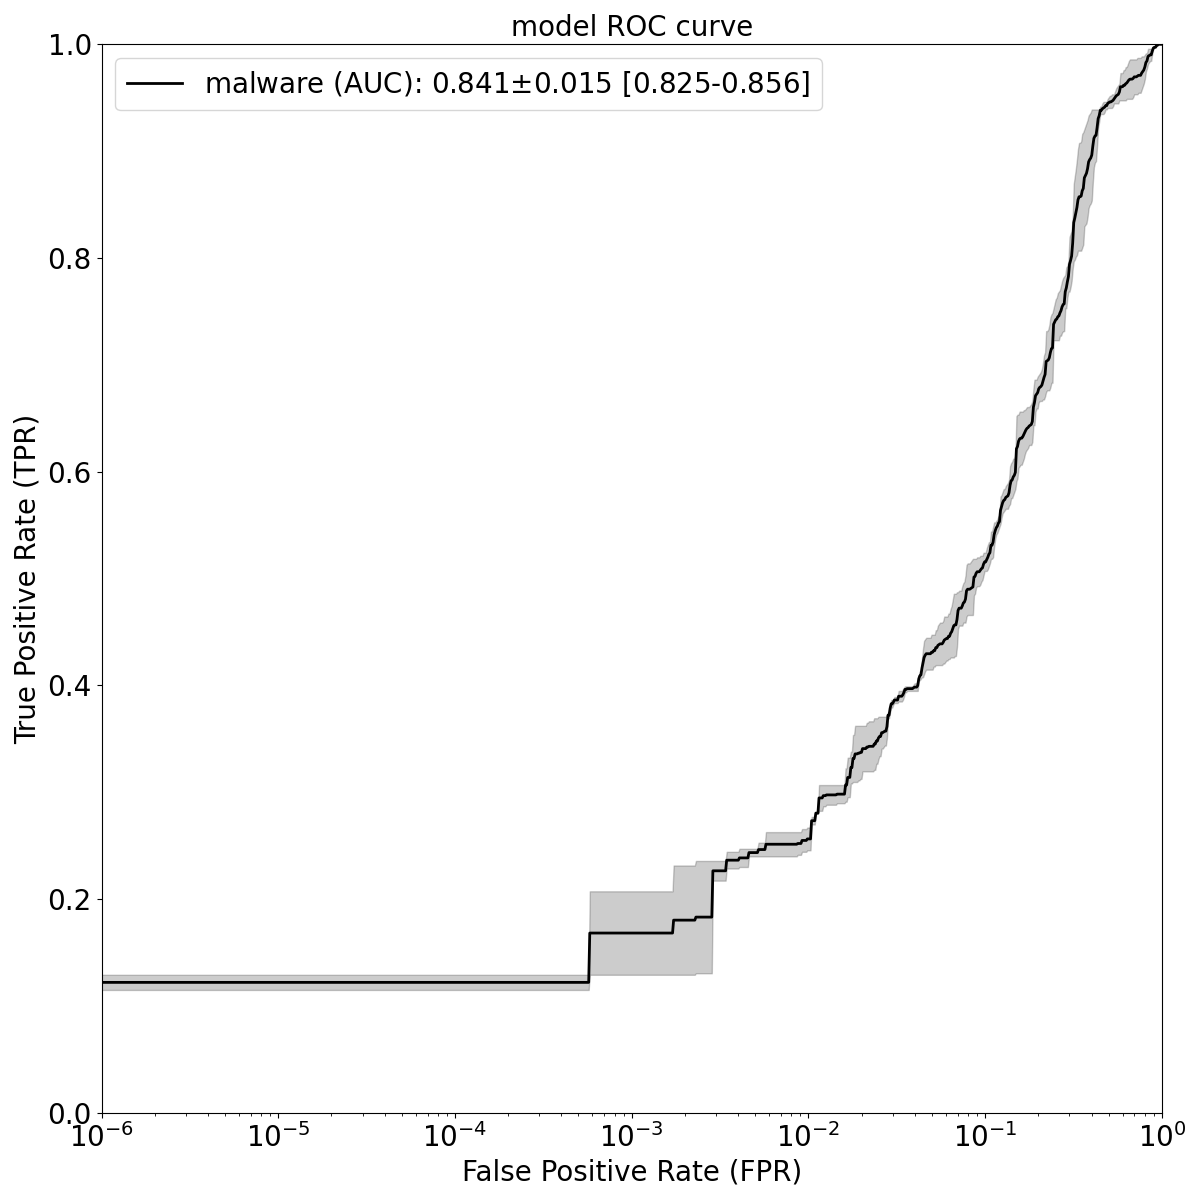
\includegraphics[width=0.6\textwidth]{./results/malware_roc_alohaMB.png}
        \vspace*{-0.2cm}
        \caption[Malware Label prediction task ALOHA (M/B only) ROC curve]{ROC curve and AUC statistics of \textBF{ALOHA (M/B only)} model for the \textbf{Malware Label}. The line represents the \textit{mean} TPR at a given FPR, while the shaded region represents the \textit{standard deviation}. Statistics were computed over \textBF{3} training runs, each with random parameter initialization.}
        \label{fig:malwareRocAlohaMB}
    \end{figure}
}

\newcommand{\malwareRocAloha}{
    \begin{figure}[h!]
        \vspace*{-0.5cm}
        \centering
        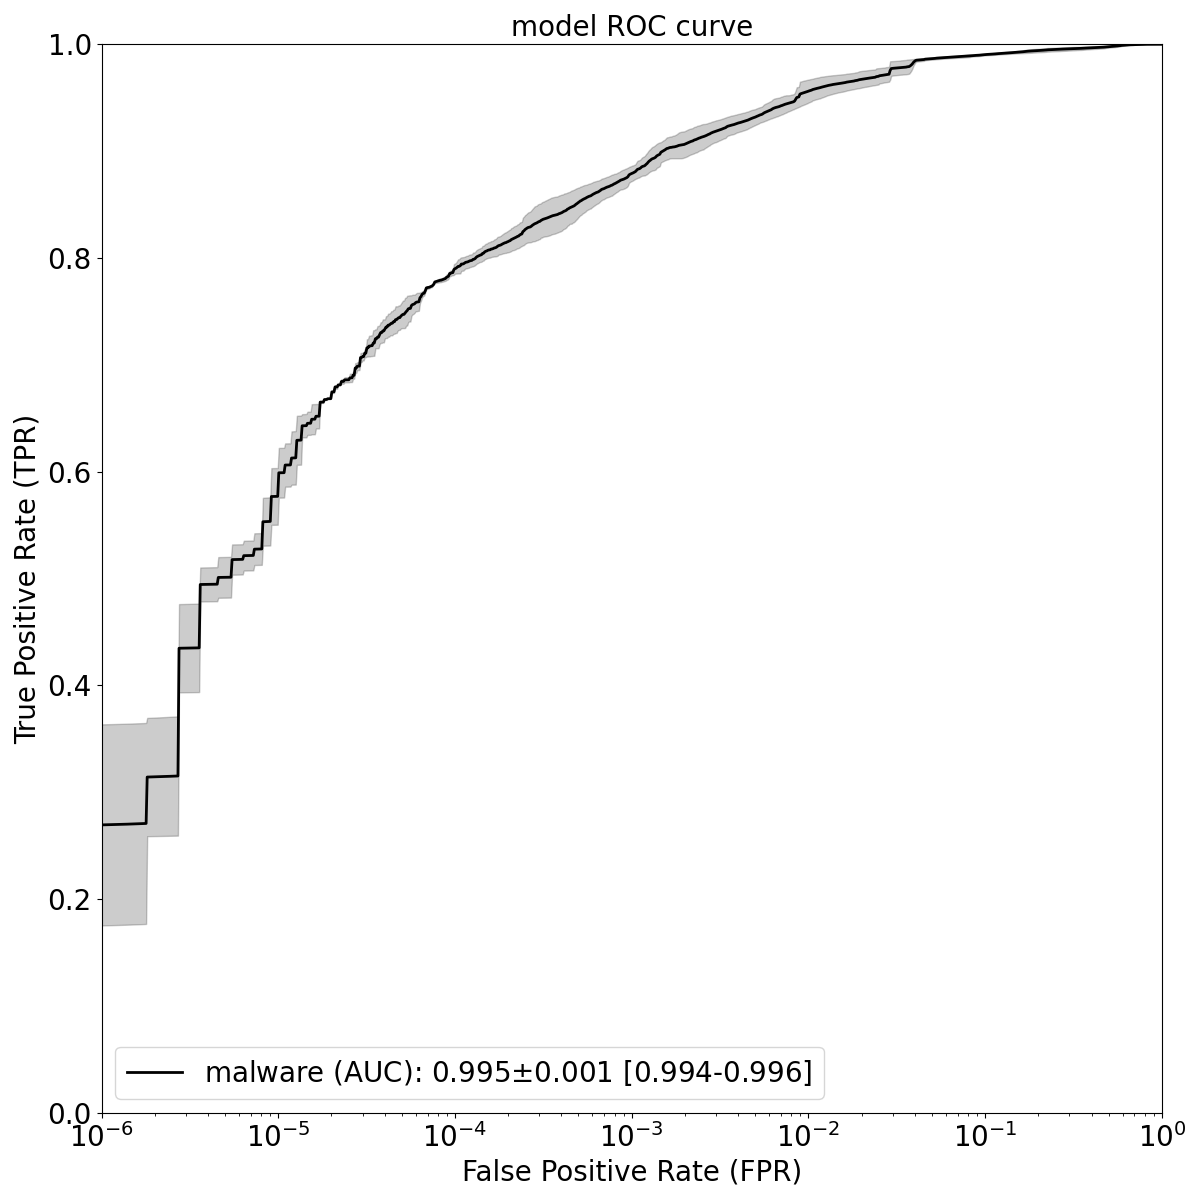
\includegraphics[width=0.6\textwidth]{./results/malware_roc_aloha.png}
        \vspace*{-0.2cm}
        \caption[Malware Label prediction task ALOHA ROC curve]{ROC curve and AUC statistics of \textBF{ALOHA} model for the \textbf{Malware Label}. The line represents the \textit{mean} TPR at a given FPR, while the shaded region represents the \textit{standard deviation}. Statistics were computed over \textBF{3} training runs, each with random parameter initialization.}
        \label{fig:malwareRocAloha}
    \end{figure}
}

\newcommand{\malwareRocJointEmbedding}{
    \begin{figure}[h!]
        \vspace*{-0.5cm}
        \centering
        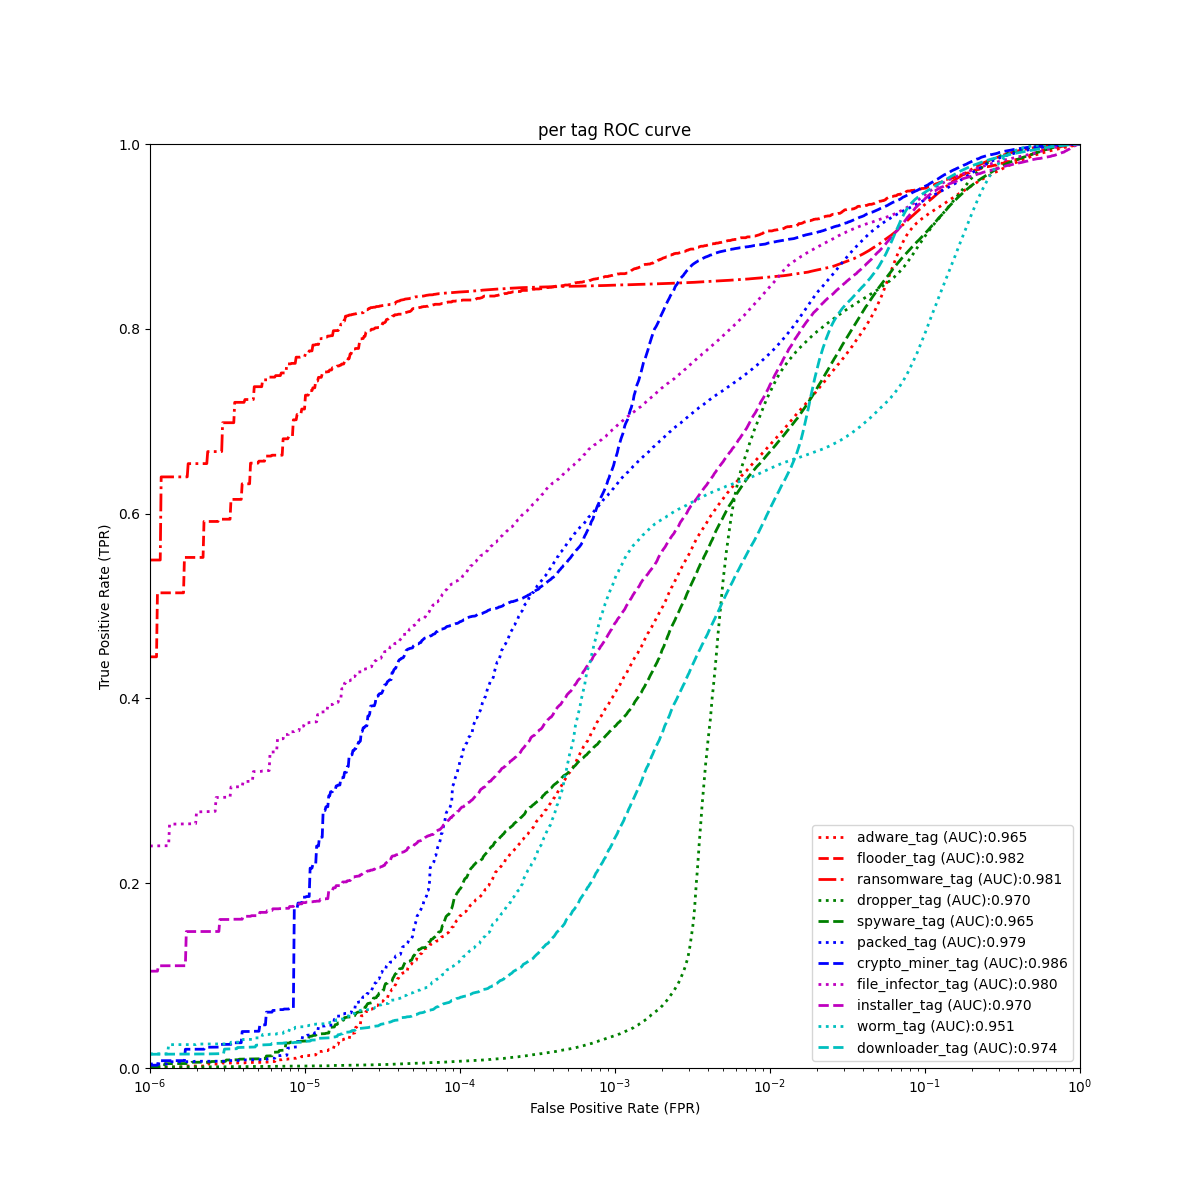
\includegraphics[width=0.6\textwidth]{./results/malware_roc_jointEmbedding.png}
        \vspace*{-0.2cm}
        \caption[Malware Label prediction task Joint Embedding ROC curve]{ROC curve and AUC statistics of \textBF{Joint Embedding} model for the \textbf{Malware Label}. The line represents the \textit{mean} TPR at a given FPR, while the shaded region represents the \textit{standard deviation}. Statistics were computed over \textBF{3} training runs, each with random parameter initialization.}
        \label{fig:malwareRocJointEmbedding}
    \end{figure}
}

\newcommand{\malwareRocProposedMethod}{
    \begin{figure}[h!]
        \vspace*{-0.5cm}
        \centering
        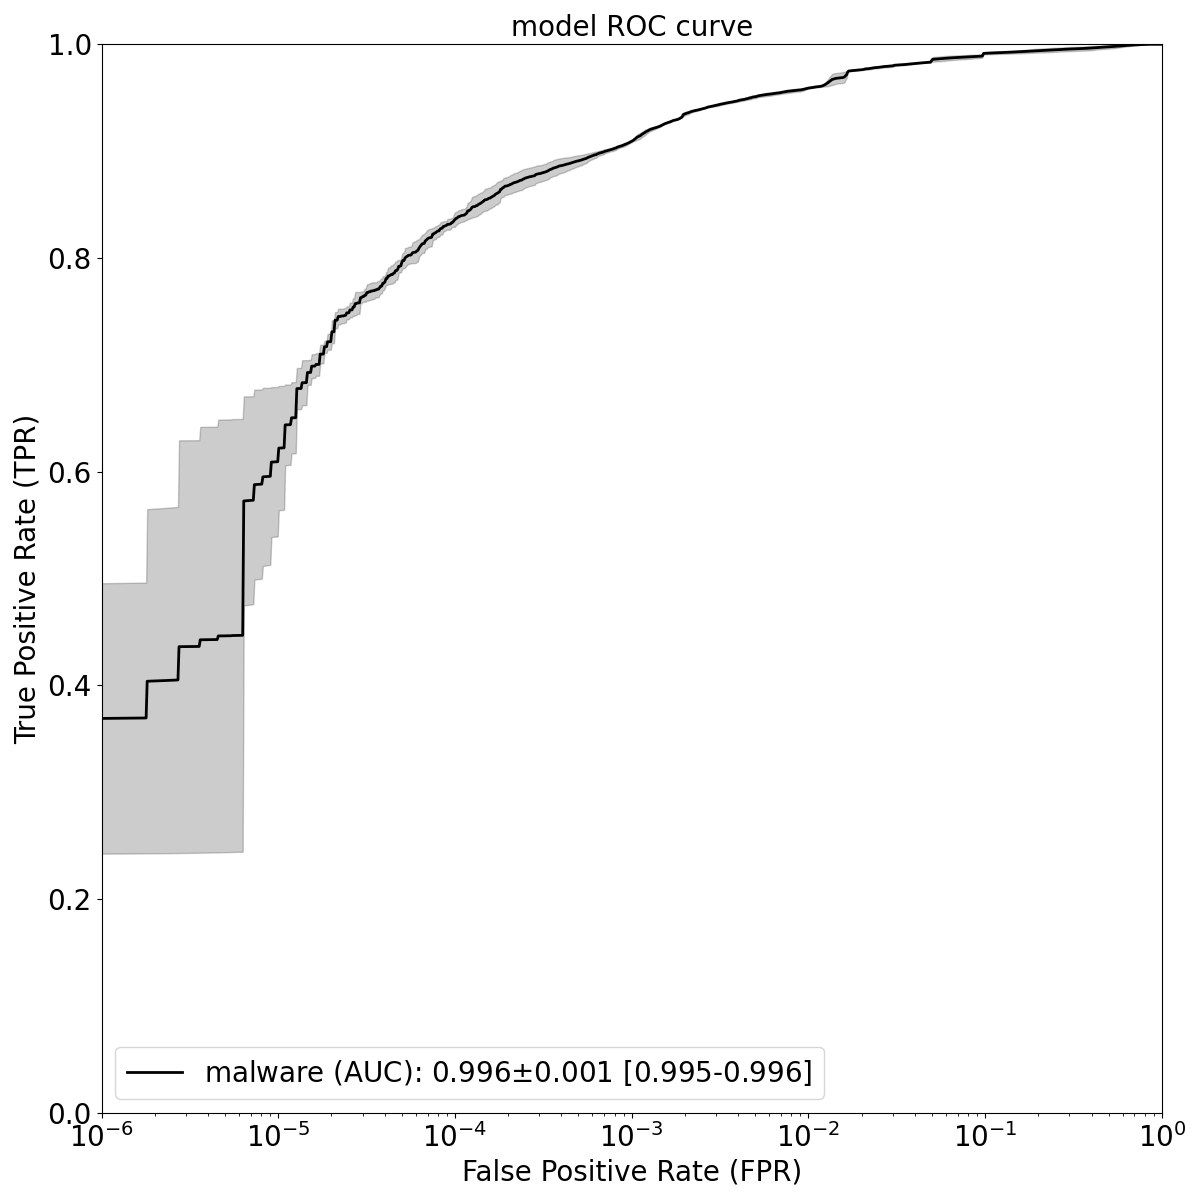
\includegraphics[width=0.6\textwidth]{./results/malware_roc_proposedModel.png}
        \vspace*{-0.2cm}
        \caption[Malware Label prediction task Proposed Model ROC curve]{ROC curve and AUC statistics of \textBF{Proposed Model} for the \textbf{Malware Label}. The line represents the \textit{mean} TPR at a given FPR, while the shaded region represents the \textit{standard deviation}. Statistics were computed over \textBF{3} training runs, each with random parameter initialization.}
        \label{fig:malwareRocProposedModel}
    \end{figure}
}
